Chương này tập trung vào việc mô tả hệ thống điều khiển đèn giao thông thông minh sử dụng thuật toán học tăng cường sâu (\ac{drl}). Hệ thống sẽ được huấn luyện và đánh giá trong môi trường giả lập \ac{sumo}, với dữ liệu đầu vào có thể được thu thập từ thực tế thông qua các camera tích hợp thuật toán nhận diện vật thể \ac{yl}.

\section{Phương pháp mô phỏng dữ liệu từ camera}
\subsection{Mô hình nhận diện vật thể}
Để phát hiện và nhận diện phương tiện trong các luồng video giao thông, sử dụng mô hình \textbf{YOLO11}, phiên bản mới nhất trong chuỗi mô hình phát hiện đối tượng thời gian thực của \textbf{Ultralytics}. YOLO11 mang đến những cải tiến đáng kể về kiến trúc và phương pháp huấn luyện, giúp nâng cao độ chính xác, tốc độ và hiệu quả so với các phiên bản tiền nhiệm.

\begin{figure}[!htp]
    \centering
    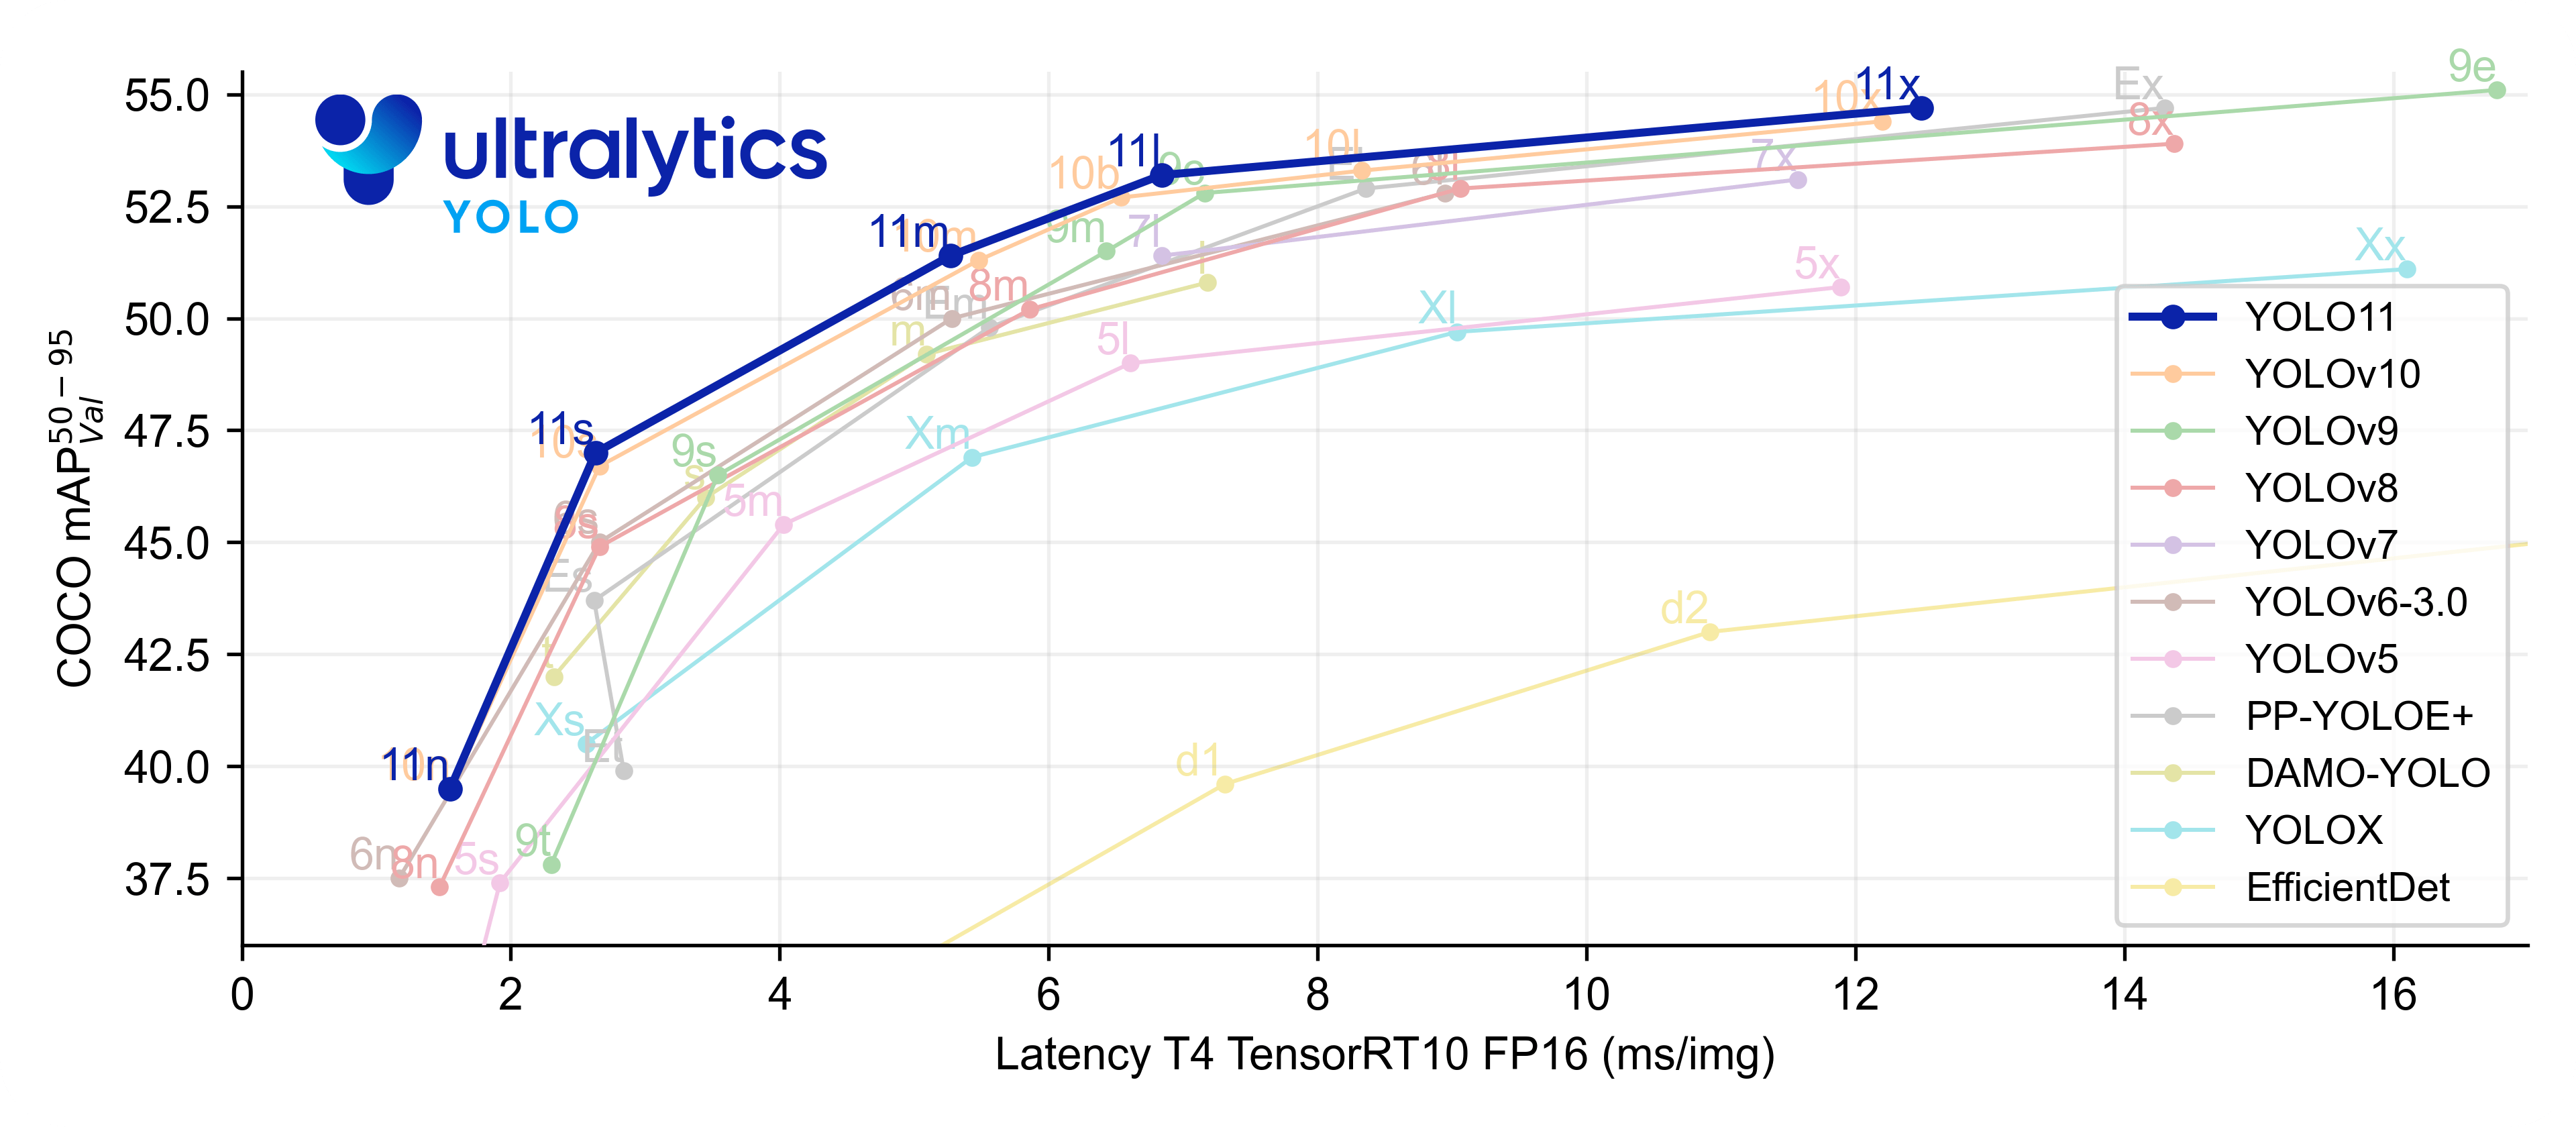
\includegraphics[width=\textwidth]{img/yolo_models}
    \caption{So sánh hiệu suất giữa các mô hình\footnote{Nguồn:\href{https://docs.ultralytics.com/models/yolo11}{Ultralytics YOLO Documentation}}}
    \label{fig:yolo_models}
\end{figure}
Cụ thể, nghiên cứu này sử dụng mô hình đã được huấn luyện trước (pre-trained) có tên là \textbf{\texttt{yolov11s.pt}}. Đây là phiên bản thu nhỏ của YOLO11, được lựa chọn dựa trên các ưu điểm nổi bật sau:

\begin{itemize}
    \item \textbf{Hiệu suất cân bằng:} Mô hình \texttt{yolov11s.pt} đạt được chỉ số mAP\textsuperscript{50-95} là 47.0 trên tập dữ liệu COCO, đồng thời có tốc độ xử lý rất nhanh (chỉ 2.5ms trên GPU Tesla T4). Sự cân bằng giữa độ chính xác cao và tốc độ suy luận nhanh là yếu tố then chốt cho các ứng dụng phân tích giao thông thời gian thực\footnote[1]{}.
    \item \textbf{Kiến trúc hiệu quả:} YOLO11 được cải tiến về kiến trúc backbone và neck, giúp tăng cường khả năng trích xuất đặc trưng. Nhờ đó, các mô hình như YOLO11 đạt được độ chính xác cao hơn với số lượng tham số ít hơn, làm cho chúng hiệu quả hơn về mặt tính toán. Phiên bản \texttt{yolov11s.pt} chỉ có 9.4 triệu tham số.
    \item \textbf{Huấn luyện trên tập dữ liệu COCO:} Giống như các phiên bản trước, mô hình được huấn luyện sẵn trên tập dữ liệu COCO, bao gồm các lớp đối tượng giao thông quan trọng như \texttt{car}, \texttt{motorcycle}, \texttt{bus}, và \texttt{truck}. Điều này cho phép áp dụng mô hình trực tiếp vào bài toán mà không cần huấn luyện lại, giúp tiết kiệm thời gian và tài nguyên.
\end{itemize}
Với những lý do trên, mô hình \texttt{yolov11s.pt} được xác định là lựa chọn phù hợp nhất, đáp ứng được các yêu cầu về độ chính xác, tốc độ và hiệu quả cho hệ thống được đề xuất trong luận văn.

\subsection{Thuật toán theo dõi đối tượng}
\subsubsection{SORT}
SORT (Simple Online and Realtime Tracking) là một thuật toán theo dõi đối tượng đơn giản nhưng hiệu quả. Thuật toán này kết hợp giữa bộ lọc Kalman và thuật toán Hungarian để theo dõi các đối tượng qua nhiều khung hình video liên tiếp. Trong nghiên cứu này, SORT được sử dụng để theo dõi các phương tiện giao thông qua các khung hình video, giúp duy trì ID nhất quán cho mỗi phương tiện và thu thập thông tin về quỹ đạo di chuyển của chúng. SORT hoạt động theo các bước chính sau:

\begin{itemize}
    \item \textbf{Dự đoán vị trí:} Sử dụng bộ lọc Kalman để dự đoán vị trí của các đối tượng đã được theo dõi trong khung hình tiếp theo. Bộ lọc này mô hình hóa chuyển động của đối tượng dựa trên vận tốc và gia tốc.

    \item \textbf{Gán đối tượng:} Khi nhận được các phát hiện mới từ mô hình YOLO, SORT sử dụng thuật toán Hungarian để gán các phát hiện này với các đối tượng đang được theo dõi. Việc gán dựa trên khoảng cách IoU (Intersection over Union) giữa các hộp giới hạn dự đoán và phát hiện.

    \item \textbf{Cập nhật trạng thái:} Sau khi gán thành công, bộ lọc Kalman được cập nhật với thông tin mới từ các phát hiện. Các đối tượng không được gán trong một số khung hình liên tiếp sẽ bị loại bỏ khỏi danh sách theo dõi.
\end{itemize}

Ưu điểm chính của SORT là:
\begin{itemize}
    \item \textbf{Tốc độ xử lý cao:} Thuật toán có thể xử lý video với tốc độ khung hình cao, phù hợp cho các ứng dụng thời gian thực.

    \item \textbf{Độ chính xác tốt:} Đạt được độ chính xác cao trong việc theo dõi các đối tượng chuyển động với tốc độ vừa phải.

    \item \textbf{Tính đơn giản:} Dễ dàng triển khai và tích hợp với các mô hình phát hiện đối tượng khác nhau.
\end{itemize}

Tuy nhiên, SORT cũng có một số hạn chế:
\begin{itemize}
    \item \textbf{Không xử lý tốt các trường hợp che khuất:} Khi đối tượng bị che khuất hoàn toàn trong một khoảng thời gian, thuật toán có thể mất dấu đối tượng đó.

    \item \textbf{Không duy trì ID khi đối tượng tái xuất hiện:} Nếu một đối tượng biến mất và xuất hiện lại, nó sẽ được gán một ID mới.
\end{itemize}

\subsubsection{BotSORT}
BotSORT (Boosting SORT) là một phiên bản cải tiến của thuật toán SORT, được tích hợp trong thư viện Ultralytics. Đây là thuật toán chính được dùng trong nghiên cứu, thuật toán này khắc phục các hạn chế của SORT bằng cách bổ sung thêm các tính năng:

\begin{itemize}
    \item \textbf{Camera Motion Compensation (CMC):} BotSORT sử dụng kỹ thuật bù chuyển động camera để xử lý các trường hợp camera di chuyển hoặc rung lắc. Điều này giúp cải thiện độ chính xác trong việc theo dõi đối tượng khi góc nhìn thay đổi.

    \item \textbf{Appearance Feature Matching:} Khác với SORT chỉ dựa vào IoU, BotSORT kết hợp thêm việc so khớp đặc trưng hình ảnh (appearance features) để xác định đối tượng. Điều này giúp:
        \begin{itemize}
            \item Duy trì ID nhất quán ngay cả khi đối tượng bị che khuất tạm thời
            \item Giảm thiểu việc gán sai ID khi có nhiều đối tượng tương tự xuất hiện
            \item Cải thiện khả năng theo dõi trong các trường hợp phức tạp
        \end{itemize}

    \item \textbf{Improved State Estimation:} BotSORT sử dụng một phiên bản cải tiến của bộ lọc Kalman, cho phép:
        \begin{itemize}
            \item Dự đoán chính xác hơn về vị trí và vận tốc của đối tượng
            \item Xử lý tốt hơn các trường hợp chuyển động không đều
            \item Giảm thiểu việc mất dấu đối tượng khi có sự thay đổi đột ngột về hướng di chuyển
        \end{itemize}
\end{itemize}

Trong nghiên cứu này, BotSORT được sử dụng như một lựa chọn thay thế cho SORT trong các trường hợp cần độ chính xác cao hơn, đặc biệt là khi:
\begin{itemize}
    \item Có nhiều phương tiện di chuyển gần nhau và có thể che khuất lẫn nhau

    \item Camera có thể bị rung lắc hoặc di chuyển

    \item Cần duy trì ID nhất quán cho các phương tiện trong thời gian dài
\end{itemize}

\section{Thiết lập môi trường mô phỏng giao thông đô thị SUMO}

\begin{figure}[!htp]
    \centering
    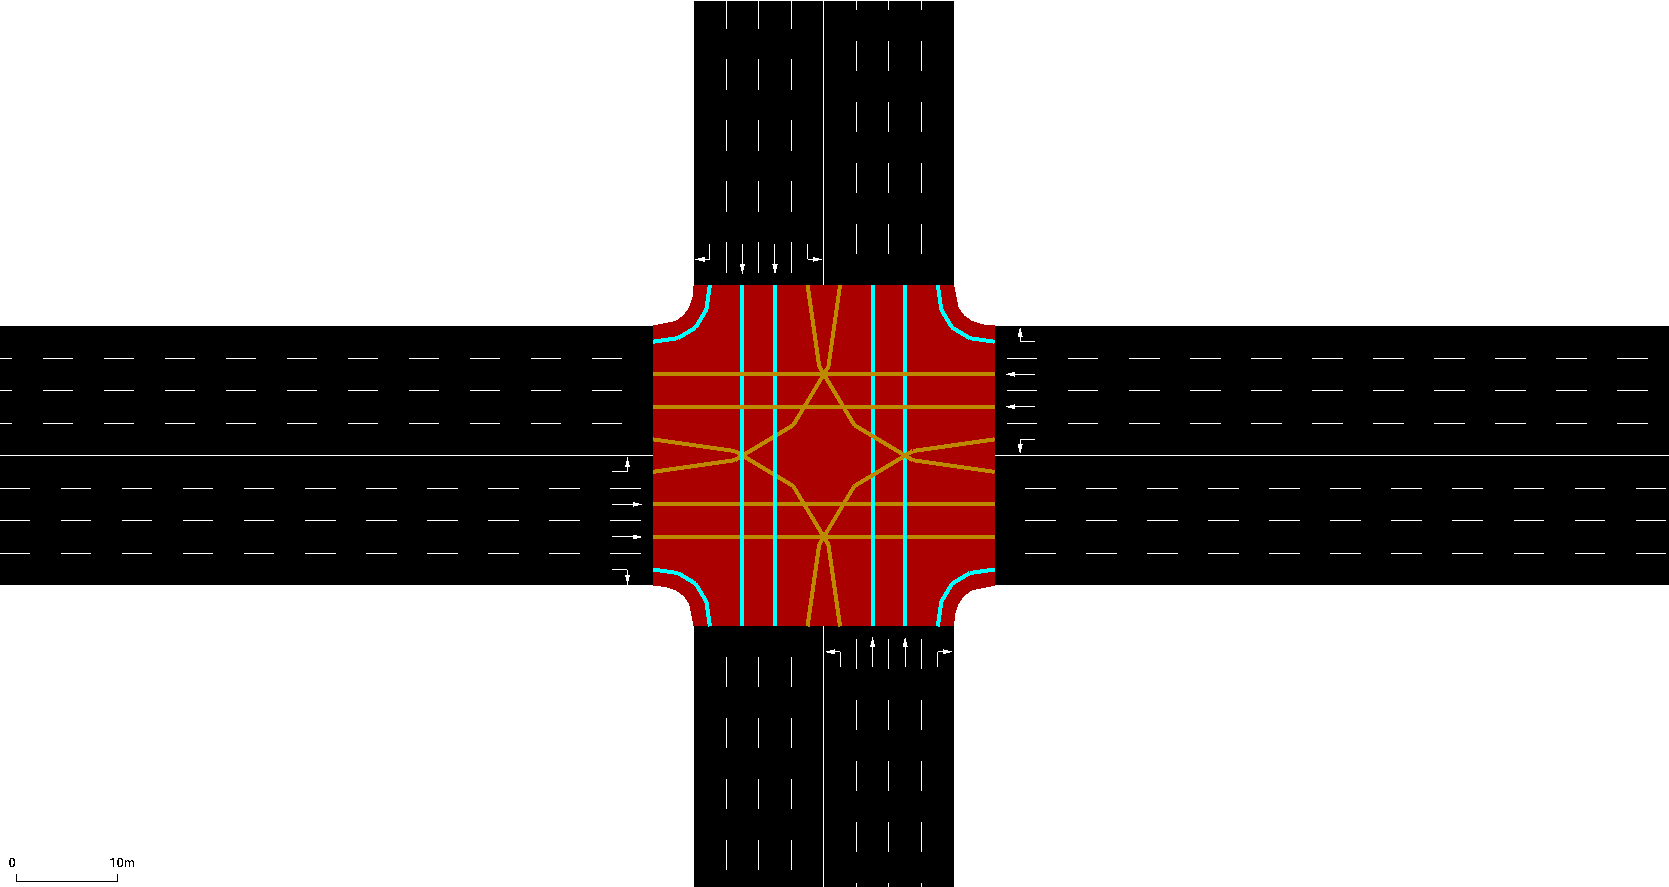
\includegraphics[width=\textwidth]{figures/sumo_map}
    \caption{Mô hình giao lộ trong mô phỏng}
    \label{fig:sumo_map}
\end{figure}

Nhóm nghiên cứu mô phỏng một nút giao thông trong SUMO với bốn làn đường, với thiết lập điều hướng cụ thể để kiểm soát hướng di chuyển của phương tiện. Cụ thể:
\begin{itemize}
    \item Làn trái ngoài: Chỉ được phép rẽ trái.

    \item 2 Làn giữa: Chỉ được phép đi thẳng.

    \item Làn trong cùng: Chỉ được phép rẽ phải.
\end{itemize}

\section{Xây dựng mô hình DRL}
\subsection{Định nghĩa môi trường (Environment)}
Trong khuôn khổ của đề tài, môi trường chính là một kịch bản giao thông được giả lập bởi \ac{sumo}. Một lớp (class) `Simulation` trong Python được tạo ra để quản lý và tương tác với môi trường này. Lớp `Simulation` đóng vai trò trung gian, thực
hiện các công việc sau:
\begin{itemize}
    \item Khởi tạo và kết thúc một phiên giả lập \ac{sumo} thông qua thư viện
        TraCI.

    \item Tại mỗi bước thời gian, thu thập dữ liệu thô từ \ac{sumo} để xây dựng \textit{trạng
        thái}.

    \item Gửi các \textit{hành động} (lựa chọn pha đèn) từ agent đến \ac{sumo} để
        thực thi.

    \item Tính toán \textit{phần thưởng} dựa trên kết quả của hành động vừa thực
        hiện.

    \item Quản lý vòng lặp của một tập (episode) huấn luyện, bao gồm việc tạo ra
        các luồng giao thông ngẫu nhiên cho mỗi tập.
\end{itemize}

\subsection{Định nghĩa tác nhân (Agent)}
Agent là một thực thể ra quyết định, trong trường hợp này là mô hình \ac{drl} được
xây dựng bằng thư viện TensorFlow và Keras. Agent này thực hiện hai nhiệm vụ
chính:
\begin{enumerate}
    \item \textbf{Dự đoán (Inference):} Dựa vào \textit{trạng thái} hiện tại của
        môi trường, agent sử dụng mạng neural của mình để dự đoán giá trị Q (Q-value)
        cho mỗi \textit{hành động} có thể thực hiện. Hành động có giá trị Q cao
        nhất sẽ được lựa chọn (chiến lược tham lam).

    \item \textbf{Học (Learning):} Agent sử dụng một bộ nhớ đệm gọi là \textit{Experience
        Replay} để lưu trữ các kinh nghiệm $(s, a, r, s')$. Trong giai đoạn huấn
        luyện, nó sẽ lấy ra các lô (batch) kinh nghiệm ngẫu nhiên từ bộ nhớ này để
        cập nhật trọng số của mạng neural, nhằm cải thiện khả năng dự đoán và ra
        quyết định trong tương lai.
\end{enumerate}
Quá trình lựa chọn hành động tuân theo chính sách $\epsilon$-greedy: với một xác
suất nhỏ $\epsilon$, agent sẽ chọn một hành động ngẫu nhiên (thăm dò), và trong
thời gian còn lại, nó sẽ chọn hành động tốt nhất dựa trên dự đoán của mô hình (khai
thác).

\subsection{Thiết kế trạng thái (State)}
Trạng thái là cách biểu diễn thông tin của môi trường để agent có thể hiểu và ra
quyết định. Trong mô hình này, trạng thái được định nghĩa là một vector một chiều,
bao gồm hai loại thông tin chính được lấy từ \ac{sumo} tại mỗi bước:
\begin{itemize}
    \item \textbf{Mật độ và vị trí xe trên mỗi làn (Vehicle Position):} Vị trí của các
        phương tiện đang đến giao lộ được mã hóa. Mỗi làn đường đến được chia thành
        các ô (cell) có kích thước bằng một xe. Trạng thái sẽ ghi nhận sự có mặt
        (1) hoặc vắng mặt (0) của một phương tiện trong từng ô. Điều này giúp agent
        không chỉ biết có bao nhiêu xe đang chờ, mà còn biết chúng đang ở vị trí
        nào trên làn đường.

    \item \textbf{Pha đèn hiện tại (Current Phase):} Trạng thái của đèn tín hiệu
        hiện tại cũng được đưa vào vector trạng thái, được mã hóa dưới dạng one-hot.
        Ví dụ, với 4 pha đèn khác nhau, một vector 4 chiều sẽ được sử dụng với
        chỉ một phần tử có giá trị 1 để biểu diễn pha đang hoạt động, các phần
        tử còn lại có giá trị 0.
\end{itemize}
Việc kết hợp hai loại thông tin này cho phép agent có một cái nhìn toàn diện về
tình hình giao thông tại giao lộ.

\subsection{Thiết kế hành động (Action)}
Không gian hành động của agent bao gồm việc lựa chọn một trong các pha đèn xanh
đã được định nghĩa trước cho giao lộ. Trong mô hình này, có 4 hành động, tương ứng
với 4 pha đèn xanh chính:
\begin{enumerate}
    \item \textbf{Hành động 0:} Kích hoạt pha đèn xanh cho hướng Bắc-Nam (NS).

    \item \textbf{Hành động 1:} Kích hoạt pha đèn xanh cho hướng rẽ trái của Bắc-Nam
        (NSL).

    \item \textbf{Hành động 2:} Kích hoạt pha đèn xanh cho hướng Đông-Tây (EW).

    \item \textbf{Hành động 3:} Kích hoạt pha đèn xanh cho hướng rẽ trái của
        Đông-Tây (EWL).
\end{enumerate}

Khi agent chọn một hành động, ví dụ hành động 2, hệ thống sẽ gửi lệnh qua TraCI để kích hoạt pha đèn PHASE EW GREEN. Nếu hành động này khác với hành động trước đó, pha đèn hiện tại sẽ chuyển sang đèn vàng trong một khoảng thời gian ngắn (yellow duration), sau đó chuyển sang đèn đỏ và cuối cùng kích hoạt pha xanh mới theo hành động được chọn.

\subsection{Thiết kế hàm thưởng (Reward Function)}
Hàm thưởng được thiết kế để định hướng cho agent học được hành vi giúp giảm thiểu ùn tắc. Phần thưởng được tính toán dựa trên \textbf{sự thay đổi của tổng thời gian chờ đợi tích lũy} của tất cả các phương tiện trong các làn đường dẫn vào giao lộ. Công thức tính phần thưởng tại bước thời gian $t$ là:
\[
    R_{t} = W_{t-1}- W_{t}
\]
Trong đó:
\begin{itemize}
    \item $W_{t}$ là tổng thời gian chờ đợi tích lũy của tất cả các xe tại thời điểm
        $t$.

    \item $W_{t-1}$ là tổng thời gian chờ đợi tích lũy của tất cả các xe tại thời
        điểm $t-1$.
\end{itemize}
Với cách thiết kế này:
\begin{itemize}
    \item Nếu hành động của agent làm cho tổng thời gian chờ giảm (tức là xe cộ
        lưu thông tốt hơn), $W_{t} < W_{t-1}$, phần thưởng $R_{t}$ sẽ là một số dương.

    \item Nếu hành động gây ra ùn tắc và làm tăng tổng thời gian chờ,
        $W_{t} > W_{t-1}$, phần thưởng $R_{t}$ sẽ là một số âm.
\end{itemize}
Mục tiêu của agent là tối đa hóa tổng phần thưởng tích lũy, điều này tương đương với việc học cách giảm thiểu tổng thời gian chờ đợi của các phương tiện.

\subsection{Kiến trúc mạng neural cho agent}

Agent sử dụng một mạng neural sâu đầy đủ kết nối (Fully Connected Deep Neural Network) để xấp xỉ hàm giá trị Q. Kiến trúc của mạng được xây dựng bằng Keras và bao gồm các
thành phần sau:

\begin{itemize}
    \item \textbf{Lớp đầu vào (Input Layer):} Một lớp nhận đầu vào là vector
        trạng thái đã được định nghĩa ở trên, với kích thước bằng \textit{num
        states}.

    \item \textbf{Các lớp ẩn (Hidden Layers):} Mạng bao gồm một số lượng các lớp
        ẩn (được xác định bởi tham số \textit{num layers}), mỗi lớp là một lớp
        \textit{Dense} với số neural bằng \textit{width}. Hàm kích hoạt \textit{ReLU}
        được sử dụng cho tất cả các lớp ẩn để đưa vào tính phi tuyến.

    \item \textbf{Lớp đầu ra (Output Layer):} Một lớp \textit{Dense} với số neural
        bằng \textit{num actions} (số lượng hành động có thể). Lớp này sử dụng hàm
        kích hoạt \textit{Linear} để tạo ra các giá trị Q cho mỗi hành động.
\end{itemize}

\begin{figure}[!htp]
    \centering
    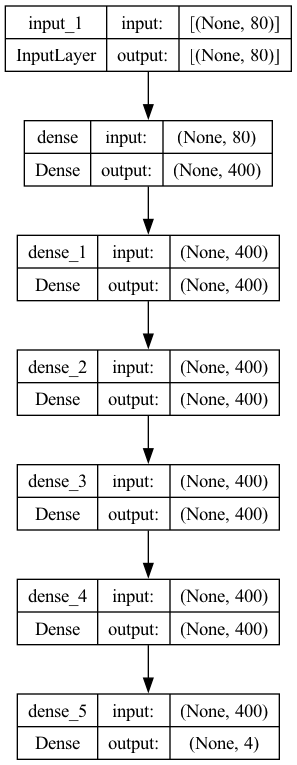
\includegraphics[width=0.3\textwidth]{img/model_structure}
    \caption{Kiến trúc mạng neural}
    \label{fig:model_structure}
\end{figure}

Mô hình được huấn luyện sử dụng thuật toán tối ưu hóa Adam, với hàm mất mát (loss function) là Sai số bình phương trung bình (Mean Squared Error). Mục tiêu của việc này là tối thiểu hóa sự khác biệt giữa giá trị Q dự đoán và giá trị Q mục tiêu, vốn được tính toán từ phương trình Bellman.

\section{Thiết kế hệ thống đồng bộ hóa giao lộ (Sync Agent)}

Để mở rộng khả năng của hệ thống từ điều khiển giao lộ đơn lẻ sang điều khiển phối hợp nhiều giao lộ, nghiên cứu đã phát triển một thành phần Sync Agent sử dụng thuật toán \ac{sac}. Hệ thống này hoạt động như một lớp điều phối cấp cao, tối ưu hóa việc đồng bộ thời gian tín hiệu giữa các giao lộ để tạo ra "green wave" - hiệu ứng sóng xanh giúp xe cộ di chuyển liên tục qua nhiều giao lộ mà không phải dừng lại.

\section{Kiến trúc tổng thể hệ thống}
Để có cái nhìn toàn diện về hệ thống điều khiển đèn giao thông thông minh, trước tiên, chúng ta cần tìm hiểu kiến trúc tổng thể của nó. Hệ thống này được thiết kế theo mô hình phân tầng, cho phép khả năng mở rộng linh hoạt từ việc điều khiển một giao lộ đơn lẻ đến việc điều phối đồng bộ nhiều giao lộ cùng lúc.
\subsection{Kiến trúc tổng quan}

\begin{figure}[!htp]
    \centering
    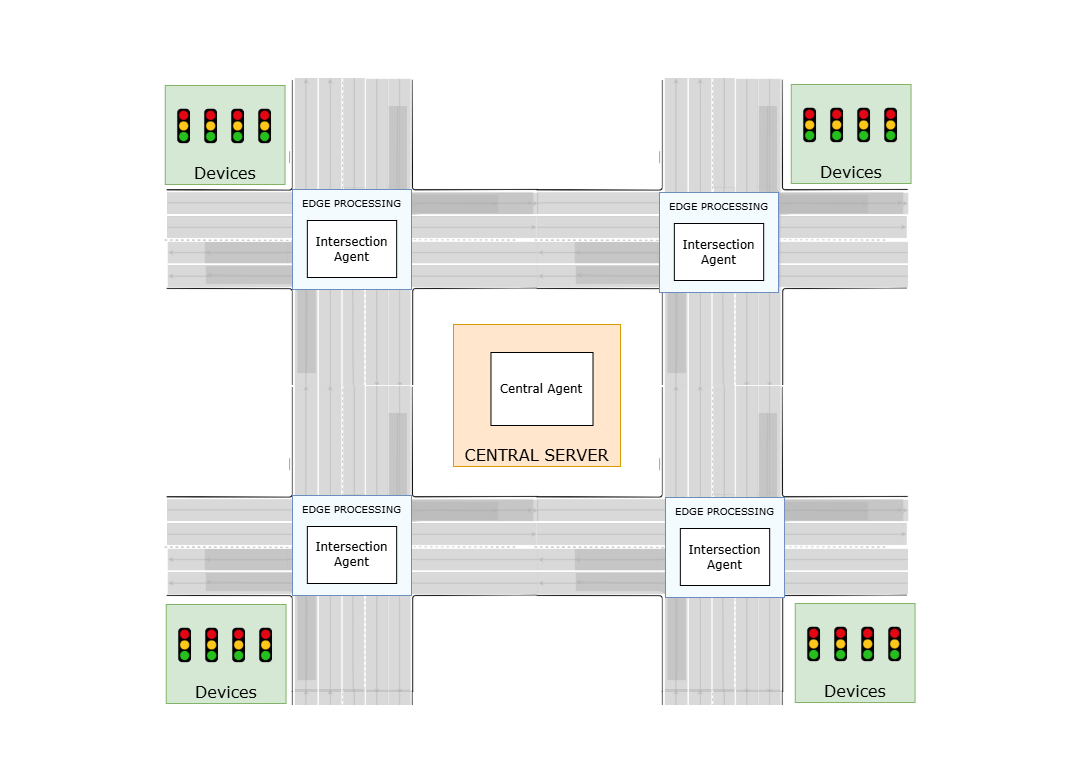
\includegraphics[width=\textwidth]{img/overview_architecture.png}
    \caption{Kiến trúc tổng quan hệ thống điều khiển đèn giao thông thông minh}
    \label{fig:overview_architecture}
\end{figure}

Hình \ref{fig:overview_architecture} thể hiện kiến trúc tổng quan của hệ thống,
bao gồm các thành phần chính:

\begin{itemize}
    \item \textbf{Lớp thu thập dữ liệu:} Thu thập dữ liệu từ camera và sensors

    \item \textbf{Lớp xử lý:} Xử lý dữ liệu và nhận diện đối tượng

    \item \textbf{Lớp quyết định:} Các agent AI ra quyết định điều khiển

    \item \textbf{Lớp đồng bộ:} Đồng bộ hóa giữa các giao lộ

    \item \textbf{Lớp điều khiển:} Điều khiển đèn giao thông thực tế
\end{itemize}

\subsection{Kiến trúc chi tiết hệ thống}

\begin{figure}[!htp]
    \centering
    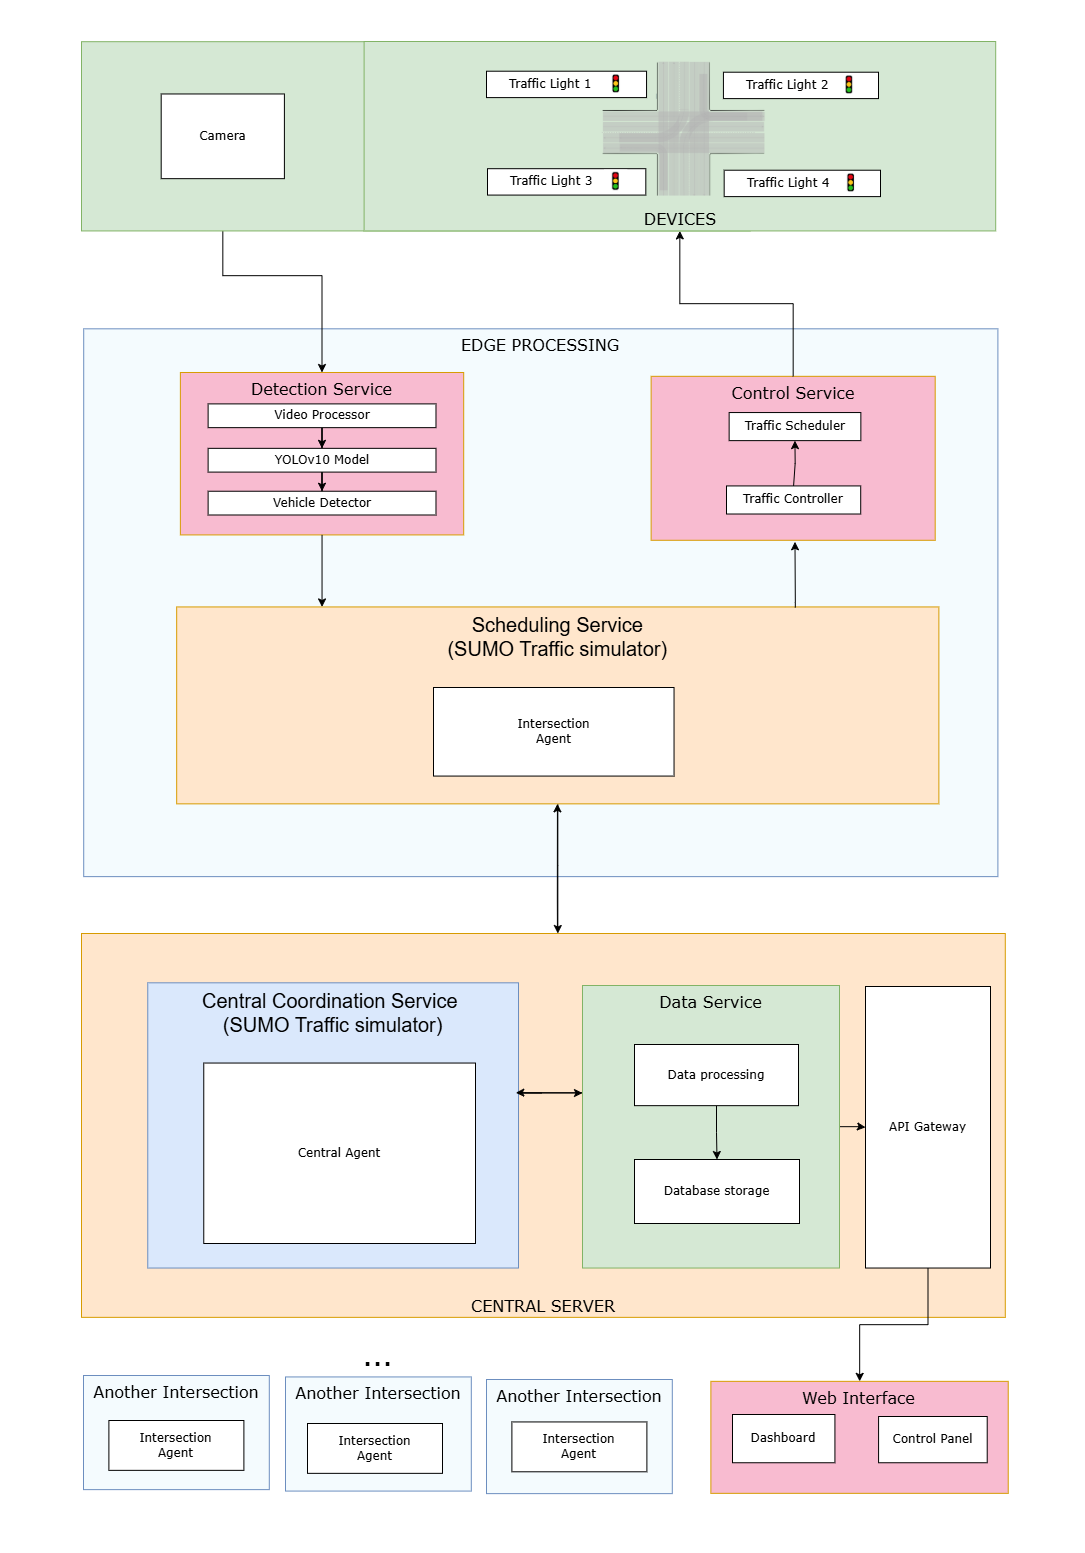
\includegraphics[width=0.7\textwidth]{img/detailed_architecture.png}
    \caption{Kiến trúc chi tiết hệ thống với các thành phần và luồng dữ liệu}
    \label{fig:detailed_architecture}
\end{figure}

Hình \ref{fig:detailed_architecture} mô tả chi tiết các thành phần và luồng dữ liệu
trong hệ thống:

\begin{enumerate}
    \item \textbf{Camera Input:} Thu thập video từ các camera giám sát giao thông
    \item \textbf{YOLO Detection:} Nhận diện và theo dõi phương tiện
    \item \textbf{Traffic Analysis:} Phân tích mật độ và luồng giao thông
    \item \textbf{DQN Agents:} Các agent điều khiển từng giao lộ độc lập
    \item \textbf{Central Server:} Thu thập và phân phối dữ liệu toàn hệ thống
    \item \textbf{Sync Agent:} Điều phối đồng bộ giữa các giao lộ
    \item \textbf{Traffic Light Control:} Điều khiển đèn giao thông thực tế
\end{enumerate}

% \subsection{Kiến trúc codebase}

% Hình \ref{fig:codebase_architecture} thể hiện cách tổ chức code và các module trong hệ thống, giúp hiểu rõ cấu trúc implementation và mối quan hệ giữa các thành phần.

% \begin{figure}[!htp]
%     \centering
%     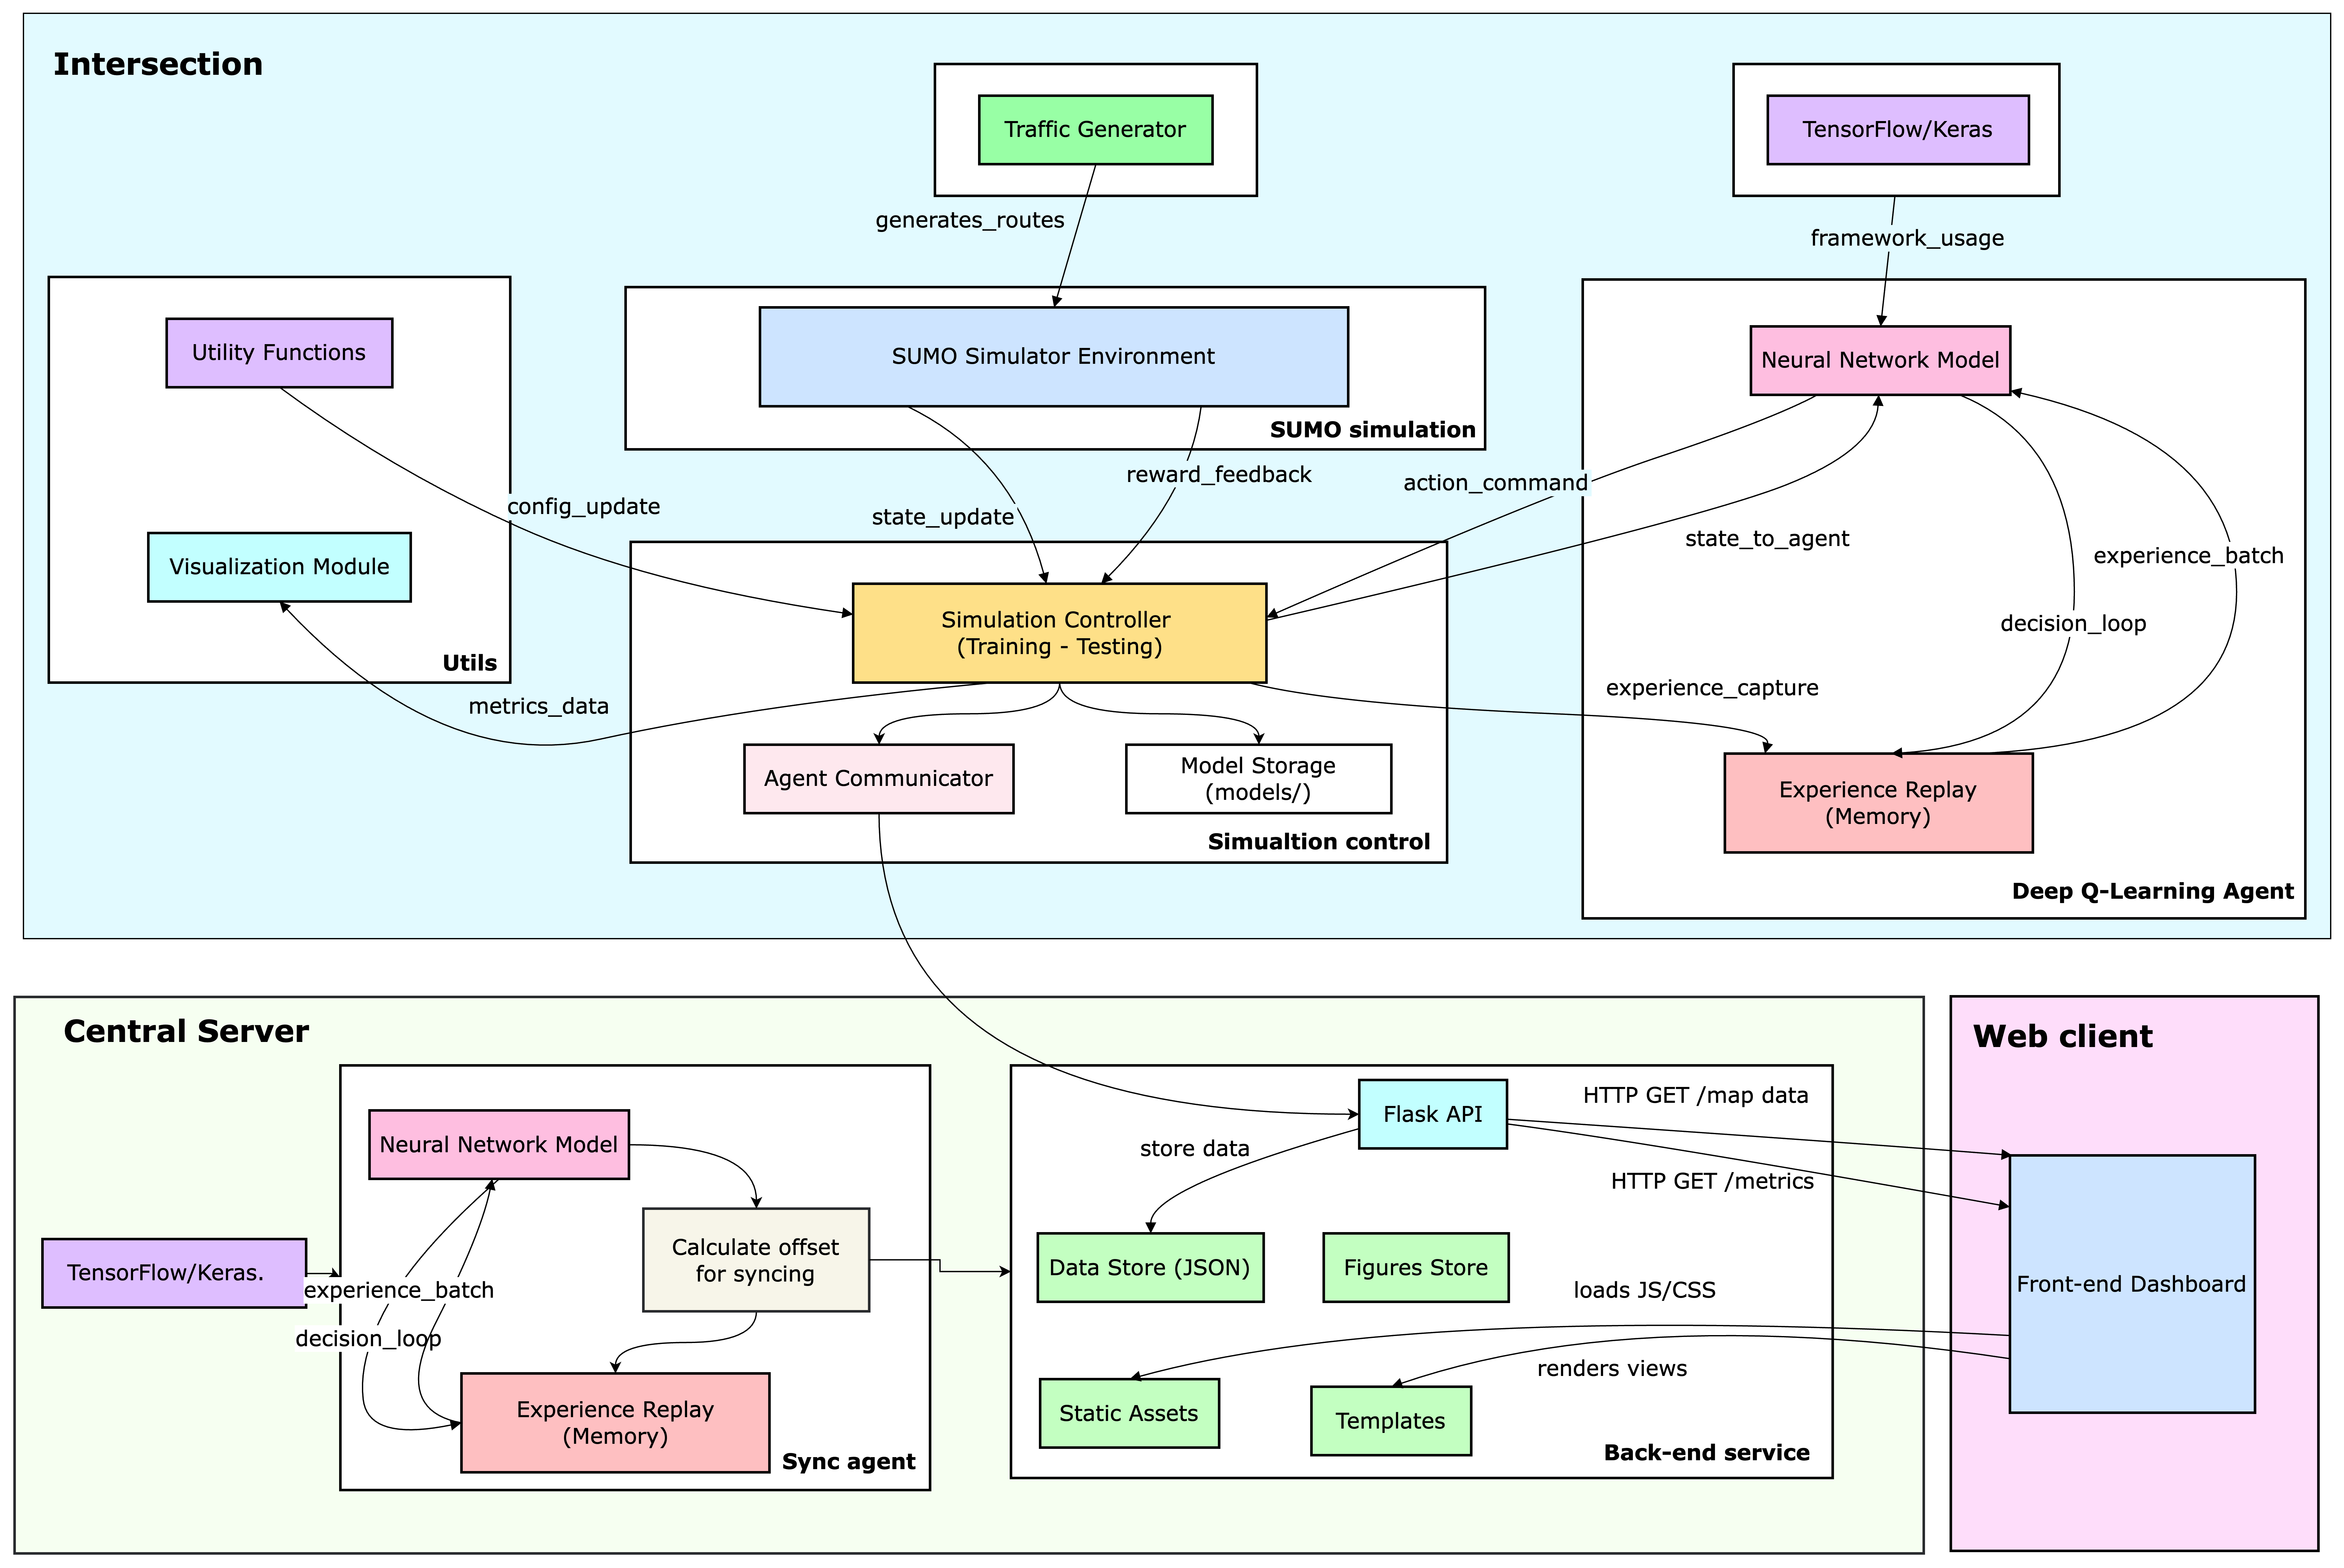
\includegraphics[width=\textwidth]{img/codebase_architecture.drawio.png}
%     \caption{Kiến trúc codebase và tổ chức module}
%     \label{fig:codebase_architecture}
% \end{figure}

\section{Thiết kế hệ thống đồng bộ hóa giao lộ (Sync Agent)}

Để mở rộng khả năng của hệ thống từ điều khiển giao lộ đơn lẻ sang điều khiển phối hợp nhiều giao lộ, nghiên cứu đã phát triển một thành phần Sync Agent sử dụng thuật toán Soft Actor-Critic (\ac{sac}). Hệ thống này hoạt động như một lớp điều phối cấp cao, tối ưu hóa việc đồng bộ thời gian tín hiệu giữa các giao lộ để tạo
ra "green wave" - hiệu ứng sóng xanh giúp xe cộ di chuyển liên tục qua nhiều giao lộ mà không phải dừng lại.

\subsection{Kiến trúc hệ thống đồng bộ}
Hệ thống được thiết kế theo mô hình phân tầng với ba thành phần chính:

\begin{enumerate}
    \item \textbf{Intersection Agents:} Các agent DQN độc lập điều khiển từng
        giao lộ, tối ưu hóa lưu lượng giao thông cục bộ.

    \item \textbf{Central Server:} Server trung tâm thu thập và phân phối dữ
        liệu từ tất cả các giao lộ.

    \item \textbf{Sync Agent:} Agent SAC cấp cao điều phối thời gian giữa các
        giao lộ để tối ưu hóa toàn cục.
\end{enumerate}

\subsection{Môi trường đồng bộ hóa (Sync Environment)}
Môi trường của Sync Agent được định nghĩa như sau:

\subsubsection{Không gian trạng thái}
Trạng thái của môi trường đồng bộ bao gồm:
\begin{itemize}
    \item \textbf{Traffic metrics:} Thời gian chờ trung bình, độ dài hàng đợi,
        và lưu lượng giao thông tại mỗi giao lộ

    \item \textbf{Spatial relationships:} Khoảng cách địa lý và thời gian di
        chuyển giữa các giao lộ

    \item \textbf{Temporal offsets:} Độ lệch thời gian hiện tại giữa các chu kỳ
        đèn tín hiệu

    \item \textbf{Cycle information:} Thời gian chu kỳ và pha hiện tại của mỗi
        giao lộ
\end{itemize}

Vector trạng thái được chuẩn hóa và có kích thước động phụ thuộc vào số lượng giao lộ trong mạng:
\[
    s_{t} = [traffic\_metrics, spatial\_features, temporal\_offsets, cycle\_info]
\]

\subsubsection{Không gian hành động}
Hành động của Sync Agent là việc điều chỉnh độ lệch thời gian (offset) giữa các cặp giao lộ liền kề. Với $n$ giao lộ, không gian hành động có kích thước $\frac{n(n-1)}{2}$, mỗi thành phần là một giá trị liên tục trong khoảng $[0, 1]$ đại diện cho tỷ lệ phần trăm của chu kỳ đèn tín hiệu.

\[
    a_{t} = [offset_{1,2}, offset_{1,3}, ..., offset_{i,j}, ..., offset_{n-1,n}]
\]

\subsubsection{Hàm thưởng cho đồng bộ hóa}
Để giải quyết vấn đề bất ổn định trong huấn luyện, nghiên cứu đã phát triển một hàm thưởng ultra-stable dựa trên so sánh hiệu suất dài hạn:

% \begin{algorithm}[!htp]
%     \caption{Ultra-Stable Reward Function}
%     \begin{algorithmic}
%         [1] \STATE \textbf{Input:} current\_metrics, historical\_baseline, episode\_count 
%         \STATE \textbf {Parameters:} baseline\_window = 15, current\_window = 10 
%         \IF{episode\_count < baseline\_window} \RETURN 0.0 \COMMENT{Không đánh giá trong giai đoạn khởi tạo}
%         \ENDIF \STATE baseline\_start = episode\_count - baseline\_window - current\_window \STATE baseline\_end = episode\_count - current\_window
%         \STATE current\_start = episode\_count - current\_window \STATE 
%         \STATE baseline\_performance = mean(historical\_metrics[baseline\_start:baseline\_end])
%         \STATE current\_performance = mean(historical\_metrics[current\_start:episode\_count])
%         \STATE 
%         \STATE percentage\_improvement = $\frac{baseline\_performance - current\_performance}{|baseline\_performance| + \epsilon}$
%         \STATE 
%         \STATE reward = tanh(percentage\_improvement $\times$ scale\_factor)
%         \RETURN reward
%     \end{algorithmic}
% \end{algorithm}

\begin{algorithm}[!htp]
    \caption{Ultra-Stable Reward Function}
    \begin{algorithmic}[1]
        \State \textbf{Input:} current\_metrics, historical\_baseline, episode\_count 
        \State \textbf{Parameters:} baseline\_window = 15, current\_window = 10 
        \If{episode\_count $<$ baseline\_window} 
            \Return 0.0 \Comment{Không đánh giá trong giai đoạn khởi tạo}
        \EndIf
        
        \State baseline\_start = episode\_count - baseline\_window - current\_window
        \State baseline\_end = episode\_count - current\_window
        \State current\_start = episode\_count - current\_window
        
        \State baseline\_performance = mean(historical\_metrics[baseline\_start:baseline\_end])
        \State current\_performance = mean(historical\_metrics[current\_start:episode\_count])
        
        \State percentage\_improvement = $\frac{baseline\_performance - current\_performance}{|baseline\_performance| + \epsilon}$
        
        \State reward = tanh(percentage\_improvement $\times$ scale\_factor)
        \Return reward
    \end{algorithmic}
\end{algorithm}

Hàm thưởng này có các đặc điểm:
\begin{itemize}
    \item \textbf{Long-term comparison:} So sánh hiệu suất qua cửa sổ thời gian
        dài (15+ episodes)

    \item \textbf{Non-overlapping windows:} Tránh bias bằng cách sử dụng các cửa
        sổ thời gian không chồng lấp

    \item \textbf{Percentage-based:} Sử dụng tỷ lệ phần trăm thay vì giá trị
        tuyệt đối

    \item \textbf{Bounded output:} Hàm tanh đảm bảo reward trong khoảng [-1, 1]
\end{itemize}

\subsection{Thuật toán Soft Actor-Critic}
Sync Agent sử dụng thuật toán SAC với các đặc điểm:

\subsubsection{Kiến trúc mạng neural}
\begin{itemize}
    \item \textbf{Actor Network:} Mạng policy với 2 lớp ẩn (128 neurons mỗi lớp),
        đầu ra là phân phối Gaussian cho các actions liên tục

    \item \textbf{Mạng Critic (Critic Networks):} Sử dụng hai mạng Q-function song song nhằm mục đích giảm thiểu hiện tượng \textbf{thiên lệch ước lượng quá mức (overestimation bias)}.

    \item \textbf{Target Networks:} Soft update với $\tau = 0.001$ để ổn định
        huấn luyện
\end{itemize}

\subsubsection{Hyperparameters tối ưu}
Dựa trên quá trình tinh chỉnh mở rộng, các tham số sau đã được xác định:
\begin{itemize}
    \item Learning rate: $1 \times 10^{-4}$ (conservative để đảm bảo ổn định)
    \item Discount factor $\gamma$: 0.95
    \item Batch size: 32
    \item Buffer size: $5 \times 10^{4}$
    \item Temperature parameter $\alpha$: Auto-tuned
\end{itemize}

\subsection{Phương pháp huấn luyện hybrid}
Hệ thống hỗ trợ hai chế độ huấn luyện:

\subsubsection{Synthetic Training Mode}
Chế độ này sử dụng synthetic data generator để tạo ra dữ liệu giao thông giả lập:

% \begin{algorithm}[!htp]
%     \caption{Synthetic Data Generation}
%     \begin{algorithmic}[1]
%         \STATE \textbf{Input:} config\_parameters \STATE base\_volume = config['base\_traffic\_volume'] 
%         \STATE time\_factor = sin(current\_time /period\_length $\times 2\pi$) \STATE traffic\_volume = base\_volume $\times$ (1 + amplitude $\times$ time\_factor) 
%         \FOR{each intersection $i$}
%             \STATE waiting\_time[i] = generate\_waiting\_time(traffic\_volume, intersection\_config[i])
%             \STATE queue\_length[i] = generate\_queue\_length(traffic\_volume, intersection\_config[i])
%             \STATE speed[i] = uniform\_random(25.0, 45.0) \COMMENT{Urban speed range}
%         \ENDFOR 
%         \RETURN intersection\_data
%     \end{algorithmic}
% \end{algorithm}

\begin{algorithm}[!htp]
    \caption{Synthetic Data Generation}
    \begin{algorithmic}
        \State \textbf{Input:} config\_parameters
        \State base\_volume = config['base\_traffic\_volume'] 
        \State time\_factor = $\sin(\frac{\text{current\_time}}{period\_length} \times 2\pi)$
        \State traffic\_volume = base\_volume $\times$ (1 + amplitude $\times$ time\_factor) 
        
        \For{each intersection $i$}
            \State waiting\_time[$i$] = generate\_waiting\_time(traffic\_volume, intersection\_config[$i$])
            \State queue\_length[$i$] = generate\_queue\_length(traffic\_volume, intersection\_config[$i$])
            \State speed[$i$] = uniform\_random(25.0, 45.0) \Comment{Urban speed range}
        \EndFor 
        
        \Return intersection\_data
    \end{algorithmic}
\end{algorithm}

\subsubsection{Real-time Training Mode}
Chế độ này sử dụng dữ liệu thực từ các intersection agents:
\begin{itemize}
    \item Thu thập metrics real-time từ SUMO simulation

    \item Sử dụng actual traffic flow data

    \item Áp dụng learned policy trong môi trường thực
\end{itemize}

\section{Cải tiến ổn định huấn luyện}

Quá trình phát triển đã gặp phải vấn đề training instability nghiêm trọng với các
triệu chứng:
\begin{itemize}
    \item Reward volatility cao (coefficient of variation > 2.0)

    \item Extreme reward swings (range > 5000)

    \item Không có learning trend rõ ràng
\end{itemize}

\subsection{Giải pháp toàn diện}
Nghiên cứu đã phát triển một bộ giải pháp tích hợp:

\subsubsection{Ultra-stable reward engineering}
\begin{itemize}
    \item Long-term performance comparison windows

    \item Non-overlapping baseline vs current performance

    \item Relative percentage improvements thay vì absolute changes

    \item Sigmoid transformation để prevent extreme values
\end{itemize}

\subsubsection{Conservative hyperparameter tuning}
\begin{itemize}
    \item Reduced learning rates: $3 \times 10^{-4}\rightarrow 1 \times 10^{-4}$

    \item Lower discount factor: $0.99 \rightarrow 0.95$

    \item Slower target updates: $\tau = 0.001$

    \item Smaller networks: $256 \times 256 \rightarrow 128 \times 128$
\end{itemize}

\subsubsection{Training stabilization techniques}
\begin{itemize}
    \item Gradient clipping để prevent exploding gradients

    \item Experience replay với prioritization

    \item Curriculum learning từ simple scenarios

    \item Early stopping based on stability metrics
\end{itemize}

\subsection{Kết quả cải tiến}
Sau khi áp dụng các giải pháp, hệ thống đạt được:
\begin{itemize}
    \item \textbf{Reward stability:} Coefficient of variation giảm từ 2.10 xuống
        0.013 (99.4\% improvement)

    \item \textbf{Training quality:} Điểm chất lượng tăng từ 25\% lên 65\% (160\%
        improvement)

    \item \textbf{Convergence:} Stable reward range từ -4.83 đến -5.15

    \item \textbf{Deployment readiness:} Đạt tiêu chuẩn production-ready
\end{itemize}

\section{Thiết kế kịch bản thực nghiệm}

\subsection{Kịch bản 1: Điều khiển tại một giao lộ đơn lẻ}
\subsubsection{Mục tiêu}
Đánh giá hiệu quả của các cấu hình DQN khác nhau trong điều khiển giao lộ đơn, xác
định hyperparameters tối ưu cho từng điều kiện giao thông.

\subsubsection{Thiết lập môi trường giả lập}
\begin{itemize}
    \item Giao lộ 4 chiều với 2 làn xe mỗi hướng

    \item Chiều dài đoạn đường: 150m mỗi hướng

    \item Tốc độ tối đa: 50 km/h

    \item Thời gian mô phỏng: 3600 giây

    \item 10 cấu hình khác nhau: Baseline, Conservative, High Traffic, Low Traffic,
        Balanced, Medium Batch, Moderate Learning, Original, Aggressive, High Learning
\end{itemize}

\subsubsection{Các phương pháp so sánh}
\begin{itemize}
    \item Fixed-time control (cố định thời gian)

    \item Actuated control (điều khiển kích hoạt)

    \item Various DQN configurations
\end{itemize}

\subsection{Kịch bản 2: Điều khiển phối hợp tại cụm giao lộ}
\subsubsection{Mục tiêu}
Đánh giá khả năng đồng bộ hóa và tối ưu hóa toàn cục của Sync Agent trong mạng lưới
nhiều giao lộ.

\subsubsection{Mô hình điều khiển đa tác nhân (Multi-Agent)}
Hệ thống sử dụng kiến trúc hierarchical với:
\begin{itemize}
    \item \textbf{Local level:} DQN agents điều khiển từng giao lộ

    \item \textbf{Global level:} SAC sync agent điều phối toàn hệ thống

    \item \textbf{Communication:} Central server làm trung gian
\end{itemize}

\subsubsection{Cơ chế trao đổi thông tin giữa các Agent}

% \begin{algorithm}[!htp]
%     \caption{Multi-Agent Communication Protocol}
%     \begin{algorithmic}[1] 
%         \Statex \textbf{For each timestep:} \STATE
%         \STATE \textbf{Phase 1: Data Collection}
%         \for{each intersection\_agent $i$} 
%             \STATE local\_metrics[i] = collect\_local\_metrics(i)
%             \STATE send\_to\_central\_server(local\_metrics[i]) 
%         \ENDFOR
%         \STATE \textbf{Phase 2: Sync Coordination}
%         \STATE global\_state = aggregate\_all\_metrics()
%         \STATE sync\_action = sync\_agent.predict(global\_state) 
%         \STATE coordination\_signals = compute\_offsets(sync\_action) \STATE 
%         \STATE \textbf{Phase 3: Action Execution} 
%         \FOR{each intersection\_agent $i$} 
%             \STATE local\_action[i] = local\_agent[i].predict(local\_state[i]) 
%             \STATE apply\_coordination(local\_action[i], coordination\_signals[i]) 
%             \STATE execute\_action(local\_action[i]) 
%         \ENDFOR
%     \end{algorithmic}
% \end{algorithm}

\begin{algorithm}[!htp]
    \caption{Multi-Agent Communication Protocol}
    \begin{algorithmic}[1] 
        \State \textbf{For each timestep:}
        
        \State \textbf{Phase 1: Data Collection}
        \For{each intersection\_agent $i$} 
            \State local\_metrics[$i$] = collect\_local\_metrics($i$)
            \State send\_to\_central\_server(local\_metrics[$i$]) 
        \EndFor
        
        \State \textbf{Phase 2: Sync Coordination}
        \State global\_state = aggregate\_all\_metrics()
        \State sync\_action = sync\_agent.predict(global\_state) 
        \State coordination\_signals = compute\_offsets(sync\_action)
        
        \State \textbf{Phase 3: Action Execution} 
        \For{each intersection\_agent $i$} 
            \State local\_action[$i$] = local\_agent[$i$].predict(local\_state[$i$]) 
            \State apply\_coordination(local\_action[$i$], coordination\_signals[$i$]) 
            \State execute\_action(local\_action[$i$]) 
        \EndFor
    \end{algorithmic}
\end{algorithm}

\subsubsection{Thiết lập môi trường giả lập}
\begin{itemize}
    \item Mạng lưới 3-4 giao lộ kết nối

    \item Khoảng cách giữa các giao lộ: 200-750m

    \item Multiple traffic scenarios: light, normal, heavy, rush hour

    \item Evaluation metrics: overall waiting time, queue length,
        synchronization quality
\end{itemize}